\chapter{Ecuaciones diferenciales lineales de orden superior}

\section{Teoría general de las EDO lineales de orden $n$}

\begin{definition}
Una \textbf{ecuación diferencial lineal de orden $n$} se escribe en su forma estándar como
\[
y^{(n)} + a_{n-1}(x)y^{(n-1)} + \cdots + a_1(x)y' + a_0(x)y = g(x),
\]
donde $a_0(x), a_1(x), \ldots, a_{n-1}(x)$ y $g(x)$ son funciones continuas en un intervalo $I$. Si $g(x) \equiv 0$, la ecuación se llama \textbf{homogénea}; en caso contrario, \textbf{no homogénea}.
\end{definition}

\begin{theorem}[Principio de superposición]\label{thm:cap28:superposicion}
Si $y_1, y_2, \ldots, y_k$ son soluciones de la ecuación homogénea
\[
y^{(n)} + a_{n-1}(x)y^{(n-1)} + \cdots + a_0(x)y = 0,
\]
entonces cualquier combinación lineal
\[
y = c_1 y_1 + c_2 y_2 + \cdots + c_k y_k
\]
también es solución.
\end{theorem}

\begin{definition}
Un conjunto de $n$ soluciones $\{y_1, y_2, \ldots, y_n\}$ de la ecuación homogénea es un \textbf{conjunto fundamental} si son linealmente independientes en $I$. La solución general de la homogénea es
\[
y_h = c_1 y_1 + c_2 y_2 + \cdots + c_n y_n.
\]
El \textbf{wronskiano} de estas funciones se define como
\[
W(y_1,\ldots,y_n)(x) =
\begin{vmatrix}
y_1 & y_2 & \cdots & y_n \\
y_1' & y_2' & \cdots & y_n' \\
\vdots & \vdots & \ddots & \vdots \\
y_1^{(n-1)} & y_2^{(n-1)} & \cdots & y_n^{(n-1)}
\end{vmatrix}.
\]
\end{definition}

\begin{theorem}[Criterio de independencia lineal]\label{thm:cap28:wronskiano}
Las soluciones $y_1,\ldots,y_n$ son linealmente independientes en $I$ si y solo si $W(y_1,\ldots,y_n)(x) \neq 0$ para todo $x \in I$.
\end{theorem}

\begin{rem}
El criterio descansa en la \textbf{fórmula de Abel}: para soluciones de la ecuación homogénea, el wronskiano satisface \(W'(x)=-a_{n-1}(x)\,W(x)\), de donde
\[
W(x)=W(x_0)\exp\!\left(-\int_{x_0}^{x} a_{n-1}(t)\,dt\right).
\]
Como la exponencial nunca se anula, \(W\) es \emph{idénticamente nula} o \emph{nunca nula} en \(I\); basta evaluarla en un punto. Si las soluciones fueran linealmente dependientes, una columna del determinante sería combinación de las otras y \(W\equiv 0\); recíprocamente, \(W(x_0)\neq 0\) impide toda relación de dependencia.
\end{rem}

\begin{theorem}[Estructura de la solución general]\label{thm:cap28:estructura}
Si $y_p$ es una solución particular de la ecuación no homogénea y $y_h$ es la solución general de la homogénea asociada, entonces la solución general de la no homogénea es
\[
y = y_h + y_p.
\]
\end{theorem}

\begin{example}[Verificación del wronskiano para dos soluciones]
Verifique que $y_1 = e^{2x}$ y $y_2 = e^{-3x}$ forman un conjunto fundamental de $y'' + y' - 6y = 0$.

\begin{myproof}
\textbf{Paso 1.} Calculamos las derivadas:
$y_1' = 2e^{2x}, y_1'' = 4e^{2x}$; $y_2' = -3e^{-3x}, y_2'' = 9e^{-3x}$.

\textbf{Paso 2.} Sustituimos en la ecuación:
Para $y_1$: $4e^{2x} + 2e^{2x} - 6e^{2x} = 0$. 
Para $y_2$: $9e^{-3x} + (-3e^{-3x}) - 6e^{-3x} = 0$. Ambas son soluciones.

\textbf{Paso 3.} Calculamos el wronskiano:
\[
W = \begin{vmatrix} e^{2x} & e^{-3x} \\ 2e^{2x} & -3e^{-3x} \end{vmatrix}
= e^{2x}(-3e^{-3x}) - e^{-3x}(2e^{2x}) = -3e^{-x} - 2e^{-x} = -5e^{-x} \neq 0.
\]

\textbf{Paso 4.} Como $W \neq 0$ para todo $x$, las funciones son linealmente independientes y forman un conjunto fundamental.

\textbf{Respuesta final:} $\boxed{\{e^{2x}, e^{-3x}\} \text{ es un conjunto fundamental.}}$
\end{myproof}
\end{example}

\begin{example}[Solución general usando superposición]
Dado que $y_1 = \cos x$ y $y_2 = \sen x$ son soluciones de $y'' + y = 0$, encuentre la solución general.

\begin{myproof}
\textbf{Paso 1.} Verificamos que ambas son soluciones: $y_1'' = -\cos x$, entonces $y_1''+y_1=0$; similar para $y_2$.

\textbf{Paso 2.} Calculamos el wronskiano:
$W = \cos x \cdot \cos x - \sen x (-\sen x) = \cos^2 x + \sen^2 x = 1 \neq 0$.

\textbf{Paso 3.} Por el principio de superposición, cualquier combinación lineal es solución. Como son linealmente independientes, forman un conjunto fundamental.

\textbf{Respuesta final:} $\boxed{y_h = c_1 \cos x + c_2 \sen x.}$
\end{myproof}
\end{example}

\begin{example}[EDO lineal de tercer orden]
Compruebe que $y_1 = 1$, $y_2 = x$, $y_3 = x^2$ son soluciones de $y''' = 0$ y halle la solución general.

\begin{myproof}
\textbf{Paso 1.} Derivadas: $y_1'=y_1''=y_1'''=0$; $y_2'=1, y_2''=0, y_2'''=0$; $y_3'=2x, y_3''=2, y_3'''=0$. Todas satisfacen $y'''=0$.

\textbf{Paso 2.} Wronskiano:
\[
W = \begin{vmatrix}
1 & x & x^2 \\
0 & 1 & 2x \\
0 & 0 & 2
\end{vmatrix} = 1 \cdot (1\cdot 2 - 2x\cdot 0) = 2 \neq 0.
\]

\textbf{Paso 3.} Son linealmente independientes, forman conjunto fundamental.

\textbf{Respuesta final:} $\boxed{y_h = c_1 + c_2 x + c_3 x^2.}$
\end{myproof}
\end{example}

\begin{example}[Ecuación no homogénea y solución general]
Si $y_p = x^2$ es una solución particular de $y'' = 2$ y la homogénea asociada es $y''=0$ con solución $y_h = c_1 + c_2 x$, escriba la solución general.

\begin{myproof}
\textbf{Paso 1.} Identificamos la homogénea: $y''=0$ tiene solución general $y_h = c_1 + c_2 x$.

\textbf{Paso 2.} Se nos da $y_p = x^2$. Verificamos: $y_p'' = 2$, correcto.

\textbf{Paso 3.} Por el teorema de estructura, la solución general es la suma.

\textbf{Respuesta final:} $\boxed{y = c_1 + c_2 x + x^2.}$
\end{myproof}
\end{example}

\section{Ecuaciones homogéneas con coeficientes constantes}

Consideramos
\[
a_n y^{(n)} + a_{n-1} y^{(n-1)} + \cdots + a_1 y' + a_0 y = 0,
\]
con $a_i \in \mathbb{R}$. Probamos soluciones de la forma $y = e^{rx}$. Sustituyendo obtenemos la \textbf{ecuación característica}:
\[
a_n r^n + a_{n-1} r^{n-1} + \cdots + a_1 r + a_0 = 0.
\]

\begin{theorem}[Casos de las raíces]
\begin{enumerate}
\item Si $r$ es raíz real simple, la solución es $e^{rx}$.
\item Si $r$ es raíz real de multiplicidad $k$, las soluciones son $e^{rx}, x e^{rx}, \ldots, x^{k-1} e^{rx}$.
\item Si $r = \alpha \pm i\beta$ es un par de raíces complejas conjugadas simples, las soluciones son $e^{\alpha x}\cos(\beta x)$ y $e^{\alpha x}\sen(\beta x)$ (las partes real e imaginaria de $e^{rx}$ vía la fórmula de Euler del Capítulo~\ref{numcomp}). Para multiplicidad $k$, se multiplican por $1, x, \ldots, x^{k-1}$.
\end{enumerate}
\end{theorem}

\begin{example}[Raíces reales distintas]
Resuelva $y'' - 5y' + 6y = 0$.

\begin{myproof}
\textbf{Paso 1.} Ecuación característica: $r^2 - 5r + 6 = 0$.

\textbf{Paso 2.} Factorizamos: $(r-2)(r-3)=0$, raíces $r=2$ y $r=3$.

\textbf{Paso 3.} Ambas reales y distintas, las soluciones son $e^{2x}$ y $e^{3x}$.

\textbf{Respuesta final:} $\boxed{y = c_1 e^{2x} + c_2 e^{3x}.}$
\end{myproof}
\end{example}

\begin{example}[Raíces reales repetidas]
Resuelva $y'' - 4y' + 4y = 0$.

\begin{myproof}
\textbf{Paso 1.} Característica: $r^2 - 4r + 4 = 0$.

\textbf{Paso 2.} Factoriza: $(r-2)^2 = 0$, raíz $r=2$ con multiplicidad 2.

\textbf{Paso 3.} Las soluciones son $e^{2x}$ y $x e^{2x}$.

\textbf{Respuesta final:} $\boxed{y = c_1 e^{2x} + c_2 x e^{2x}.}$
\end{myproof}
\end{example}

\begin{example}[Raíces complejas conjugadas]
Resuelva $y'' + 2y' + 5y = 0$.

\begin{myproof}
\textbf{Paso 1.} Característica: $r^2 + 2r + 5 = 0$.

\textbf{Paso 2.} Fórmula cuadrática: $r = \frac{-2 \pm \sqrt{4-20}}{2} = \frac{-2 \pm 4i}{2} = -1 \pm 2i$.

\textbf{Paso 3.} Aquí $\alpha = -1$, $\beta = 2$. Las soluciones son $e^{-x}\cos(2x)$ y $e^{-x}\sen(2x)$.

\textbf{Respuesta final:} $\boxed{y = e^{-x}(c_1 \cos 2x + c_2 \sen 2x).}$
\end{myproof}
\end{example}

\begin{example}[Ecuación de tercer orden con raíces mixtas]
Resuelva $y''' - 3y'' + 3y' - y = 0$.

\begin{myproof}
\textbf{Paso 1.} Característica: $r^3 - 3r^2 + 3r - 1 = 0$.

\textbf{Paso 2.} Identificamos $(r-1)^3 = 0$, raíz $r=1$ multiplicidad 3.

\textbf{Paso 3.} Las soluciones son $e^{x}, x e^{x}, x^2 e^{x}$.

\textbf{Respuesta final:} $\boxed{y = e^{x}(c_1 + c_2 x + c_3 x^2).}$
\end{myproof}
\end{example}

\section{Método de coeficientes indeterminados}

Para ecuaciones no homogéneas con coeficientes constantes:
\[
a_n y^{(n)} + \cdots + a_0 y = g(x),
\]
donde $g(x)$ es una combinación de polinomios, exponenciales, senos y cosenos, proponemos una solución particular $y_p$ con coeficientes indeterminados.

\begin{definition}[Tabla de formas de $y_p$]
\begin{center}
\begin{tabular}{c|c}
$g(x)$ & Forma de $y_p$ \\ \hline
$P_n(x)$ (polinomio de grado $n$) & $x^s (A_n x^n + \cdots + A_0)$ \\
$P_n(x) e^{\alpha x}$ & $x^s e^{\alpha x}(A_n x^n + \cdots + A_0)$ \\
$P_n(x) e^{\alpha x}\cos(\beta x)$ & $x^s e^{\alpha x}[(A_n x^n + \cdots + A_0)\cos(\beta x) + (B_n x^n + \cdots + B_0)\sen(\beta x)]$ \\
\end{tabular}
\end{center}
donde $s$ es el menor entero no negativo tal que ningún término de $y_p$ sea solución de la homogénea asociada.
\end{definition}

\begin{example}[Término forzado polinomial]
Resuelva $y'' - 3y' + 2y = 2x^2$.

\begin{myproof}
\textbf{Paso 1.} Homogénea: $r^2 - 3r + 2 = 0 \Rightarrow r=1,2$, $y_h = c_1 e^x + c_2 e^{2x}$.

\textbf{Paso 2.} Como $g(x)=2x^2$ (polinomio grado 2), proponemos $y_p = Ax^2 + Bx + C$. Ningún término solapa con $y_h$.

\textbf{Paso 3.} Derivamos: $y_p' = 2Ax + B$, $y_p'' = 2A$. Sustituimos:
$2A - 3(2Ax+B) + 2(Ax^2+Bx+C) = 2x^2$.
Agrupamos: $2A x^2 + (-6A+2B)x + (2A - 3B + 2C) = 2x^2$.

\textbf{Paso 4.} Igualamos coeficientes:
$2A = 2 \Rightarrow A=1$; $-6A+2B=0 \Rightarrow -6+2B=0 \Rightarrow B=3$; $2A - 3B + 2C = 0 \Rightarrow 2 - 9 + 2C = 0 \Rightarrow C = 7/2$.

\textbf{Paso 5.} $y_p = x^2 + 3x + 7/2$.

\textbf{Respuesta final:} $\boxed{y = c_1 e^x + c_2 e^{2x} + x^2 + 3x + \frac{7}{2}.}$
\end{myproof}
\end{example}

\begin{example}[Término exponencial]
Resuelva $y'' - 5y' + 6y = 4e^{3x}$.

\begin{myproof}
\textbf{Paso 1.} Homogénea: $r^2 - 5r + 6 = 0 \Rightarrow r=2,3$, $y_h = c_1 e^{2x} + c_2 e^{3x}$.

\textbf{Paso 2.} $g(x)=4e^{3x}$. La forma básica es $A e^{3x}$, pero $e^{3x}$ es solución de la homogénea ($r=3$). Multiplicamos por $x$: $y_p = A x e^{3x}$.

\textbf{Paso 3.} Derivamos: $y_p' = A e^{3x}(1+3x)$, $y_p'' = A e^{3x}(6+9x)$.

\textbf{Paso 4.} Sustituimos:
$A e^{3x}(6+9x) - 5A e^{3x}(1+3x) + 6A x e^{3x} = 4e^{3x}$.
Factor $A e^{3x}$: $(6+9x - 5 -15x + 6x) = (1 + 0x) = 1$. Entonces $A = 4$.

\textbf{Respuesta final:} $\boxed{y = c_1 e^{2x} + c_2 e^{3x} + 4x e^{3x}.}$
\end{myproof}
\end{example}

\begin{example}[Término seno/coseno]
Resuelva $y'' + y = 3\sen(2x)$.

\begin{myproof}
\textbf{Paso 1.} Homogénea: $r^2+1=0 \Rightarrow r=\pm i$, $y_h = c_1 \cos x + c_2 \sen x$.

\textbf{Paso 2.} $g(x)=3\sen(2x)$. Proponemos $y_p = A\cos(2x) + B\sen(2x)$ (no solapa).

\textbf{Paso 3.} Derivadas: $y_p' = -2A\sen(2x)+2B\cos(2x)$; $y_p'' = -4A\cos(2x)-4B\sen(2x)$.

\textbf{Paso 4.} Sustituimos: $(-4A\cos -4B\sen) + (A\cos + B\sen) = -3A\cos -3B\sen = 3\sen(2x)$.
Igualamos: $-3A = 0 \Rightarrow A=0$; $-3B = 3 \Rightarrow B=-1$.

\textbf{Respuesta final:} $\boxed{y = c_1 \cos x + c_2 \sen x - \sen(2x).}$
\end{myproof}
\end{example}

\begin{example}[Producto de exponencial y polinomio]
Resuelva $y'' - 2y' + y = e^x (x+1)$.

\begin{myproof}
\textbf{Paso 1.} Homogénea: $r^2 - 2r + 1 = (r-1)^2=0$, $y_h = c_1 e^x + c_2 x e^x$.

\textbf{Paso 2.} $g(x)=e^x(x+1)$. Forma básica: $e^x(Ax+B)$. Pero $e^x$ y $x e^x$ son soluciones de la homogénea, así que multiplicamos por $x^2$: $y_p = x^2 e^x (Ax+B) = e^x(Ax^3 + Bx^2)$.

\textbf{Paso 3.} Derivamos (usamos $y_p = e^x (Ax^3+Bx^2)$):
$y_p' = e^x[Ax^3 + (3A+B)x^2 + 2Bx]$.
$y_p'' = e^x[Ax^3 + (6A+B)x^2 + (6A+4B)x + 2B]$.

\textbf{Paso 4.} Sustituimos en $y'' -2y' + y$:
$e^x[ (Ax^3+(6A+B)x^2+(6A+4B)x+2B) - 2(Ax^3+(3A+B)x^2+2Bx) + (Ax^3+Bx^2) ]$.
Simplificamos coeficientes:
$x^3: A-2A+A=0$.
$x^2: (6A+B) - 2(3A+B) + B = 6A+B-6A-2B+B = 0$.
$x: (6A+4B) - 4B = 6A$.
constante: $2B$.
Entonces $e^x(6A x + 2B) = e^x(x+1)$.
Igualamos: $6A=1 \Rightarrow A=1/6$; $2B=1 \Rightarrow B=1/2$.

\textbf{Respuesta final:} $\boxed{y = c_1 e^x + c_2 x e^x + e^x\left(\frac{1}{6}x^3 + \frac{1}{2}x^2\right).}$
\end{myproof}
\end{example}

\begin{example}[Coeficientes indeterminados con resonancia]
Resuelva $y'' + 9y = \cos(3x)$.

\begin{myproof}
\textbf{Paso 1.} Homogénea: $r^2+9=0 \Rightarrow r=\pm 3i$, luego $y_h=c_1\cos 3x+c_2\sen 3x$.

\textbf{Paso 2.} El término $g(x)=\cos 3x$ \emph{ya está} en $y_h$ (resonancia), así que multiplicamos por $x$ y proponemos $y_p=x(A\cos 3x+B\sen 3x)$.

\textbf{Paso 3.} Derivando y sustituyendo se obtiene $y_p''+9y_p=-6A\sen 3x+6B\cos 3x$. Igualando a $\cos 3x$: $-6A=0$ y $6B=1$, de donde $A=0$, $B=\frac{1}{6}$.

\textbf{Respuesta final:} $\boxed{y=c_1\cos 3x+c_2\sen 3x+\frac{1}{6}x\sen 3x.}$
\end{myproof}
\end{example}

\section{Método de variación de parámetros}

Este método funciona para cualquier $g(x)$ continua. Para una EDO lineal de segundo orden en forma estándar:
\[
y'' + P(x)y' + Q(x)y = g(x),
\]
si $y_1, y_2$ forman un conjunto fundamental de la homogénea, buscamos $y_p = u_1(x) y_1 + u_2(x) y_2$ con
\[
u_1' = -\frac{g(x) y_2}{W}, \qquad u_2' = \frac{g(x) y_1}{W},
\]
donde $W = y_1 y_2' - y_2 y_1'$.

\begin{example}[$g(x) = \sec x$]
Resuelva $y'' + y = \sec x$.

\begin{myproof}
\textbf{Paso 1.} Homogénea: $y''+y=0$, $y_1=\cos x$, $y_2=\sen x$, $W = 1$.

\textbf{Paso 2.} $g(x)=\sec x = 1/\cos x$. Entonces:
$u_1' = -\frac{g y_2}{W} = -\frac{\sec x \cdot \sen x}{1} = -\tan x$.
$u_2' = \frac{g y_1}{W} = \frac{\sec x \cdot \cos x}{1} = 1$.

\textbf{Paso 3.} Integramos: $u_1 = -\int \tan x \, dx = -\ln|\sec x| + C_1$ (omitimos constantes); $u_2 = \int 1 \, dx = x$.

\textbf{Paso 4.} $y_p = u_1 y_1 + u_2 y_2 = -\ln|\sec x| \cos x + x \sen x$.

\textbf{Respuesta final:} $\boxed{y = c_1 \cos x + c_2 \sen x - \cos x \ln|\sec x| + x \sen x.}$
\end{myproof}
\end{example}

\begin{example}[$g(x) = \ln x$]
Resuelva $x^2 y'' - 2x y' + 2y = x^2 \ln x$ (forma estándar: $y'' - \frac{2}{x}y' + \frac{2}{x^2}y = \ln x$).

\begin{myproof}
\textbf{Paso 1.} Primero hallamos $y_1, y_2$ para la homogénea $x^2 y'' - 2x y' + 2y = 0$. Probamos $y=x^m$: $m(m-1)-2m+2 = m^2 -3m+2 = (m-1)(m-2)=0$, $y_1=x, y_2=x^2$.

\textbf{Paso 2.} Escribimos en forma estándar: $y'' - \frac{2}{x}y' + \frac{2}{x^2}y = \ln x$, así $g(x)=\ln x$. $W = x(2x) - x^2(1) = x^2$.

\textbf{Paso 3.} $u_1' = -\frac{g y_2}{W} = -\frac{\ln x \cdot x^2}{x^2} = -\ln x$; $u_2' = \frac{g y_1}{W} = \frac{\ln x \cdot x}{x^2} = \frac{\ln x}{x}$.

\textbf{Paso 4.} Integramos: $u_1 = -\int \ln x \, dx = -x\ln x + x$; $u_2 = \int \frac{\ln x}{x} dx = \frac{1}{2}(\ln x)^2$.

\textbf{Paso 5.} $y_p = u_1 x + u_2 x^2 = (-x\ln x + x)x + \frac{1}{2}(\ln x)^2 x^2 = -x^2\ln x + x^2 + \frac{x^2}{2}(\ln x)^2$.

\textbf{Respuesta final:} $\boxed{y = c_1 x + c_2 x^2 + x^2\left(1 - \ln x + \frac{1}{2}(\ln x)^2\right).}$
\end{myproof}
\end{example}

\begin{example}[$g(x) = e^x$ con coeficientes variables]
Resuelva $y'' - 2y' + y = \frac{e^x}{x}$.

\begin{myproof}
\textbf{Paso 1.} Homogénea: $r^2 - 2r + 1=0$, $y_1=e^x$, $y_2=x e^x$. $W = e^x(e^x + x e^x) - x e^x (e^x) = e^{2x}$.

\textbf{Paso 2.} $g(x) = e^x/x$. Entonces:
$u_1' = -\frac{g y_2}{W} = -\frac{(e^x/x)(x e^x)}{e^{2x}} = -1/x$.
$u_2' = \frac{g y_1}{W} = \frac{(e^x/x)(e^x)}{e^{2x}} = 1/x$.

\textbf{Paso 3.} Integramos: $u_1 = -\ln|x|$; $u_2 = \ln|x|$.

\textbf{Paso 4.} $y_p = u_1 e^x + u_2 x e^x = -e^x \ln|x| + x e^x \ln|x| = e^x (x-1)\ln|x|$.

\textbf{Respuesta final:} $\boxed{y = c_1 e^x + c_2 x e^x + e^x(x-1)\ln|x|.}$
\end{myproof}
\end{example}

\begin{example}[$g(x) = \tan x$]
Resuelva $y'' + 4y = \tan(2x)$.

\begin{myproof}
\textbf{Paso 1.} Homogénea: $r^2+4=0 \Rightarrow r=\pm 2i$, $y_1=\cos 2x$, $y_2=\sen 2x$. $W = 2$ (constante).

\textbf{Paso 2.} $g(x)=\tan(2x)$. Entonces:
$u_1' = -\frac{g y_2}{W} = -\frac{\tan(2x) \sen(2x)}{2} = -\frac{\sen^2(2x)}{2\cos(2x)}$.
$u_2' = \frac{g y_1}{W} = \frac{\tan(2x) \cos(2x)}{2} = \frac{\sen(2x)}{2}$.

\textbf{Paso 3.} Integramos $u_2 = -\frac{1}{4}\cos(2x)$. Para $u_1$: sustituimos $t=2x$ en $\int\!\frac{\sen^2(2x)}{2\cos(2x)}\,dx = \frac{1}{4}\!\int\!\frac{\sen^2 t}{\cos t}\,dt = \frac{1}{4}\!\int\!(\sec t-\cos t)\,dt = \frac{1}{4}[\ln|\sec t+\tan t|-\sen t]$. Por tanto $u_1 = -\frac{1}{4}[\ln|\sec(2x)+\tan(2x)|-\sen(2x)]$.

\textbf{Paso 4.} $y_p = u_1\cos 2x + u_2\sen 2x = -\tfrac{1}{4}[\ln|\sec(2x)+\tan(2x)|-\sen(2x)]\cos(2x) - \tfrac{\cos(2x)}{4}\sen(2x) = -\tfrac{1}{4}\cos(2x)\ln|\sec(2x)+\tan(2x)|$.

\textbf{Respuesta final:} $\boxed{y = c_1 \cos 2x + c_2 \sen 2x - \frac{1}{4}\cos 2x\ln|\sec 2x + \tan 2x|.}$
\end{myproof}
\end{example}

\begin{example}[Variación de parámetros con $\tan x$]
Resuelva $y'' + y = \tan x$.

\begin{myproof}
\textbf{Paso 1.} Homogénea: $y_1=\cos x$, $y_2=\sen x$, con wronskiano $W=\cos^2 x+\sen^2 x=1$.

\textbf{Paso 2.} Fórmulas de variación de parámetros:
\[
u_1'=-\frac{y_2\,g}{W}=-\sen x\tan x=-\frac{\sen^2 x}{\cos x}=-(\sec x-\cos x),\qquad
u_2'=\frac{y_1\,g}{W}=\cos x\tan x=\sen x.
\]

\textbf{Paso 3.} Integrar:
\[
u_1=-\ln|\sec x+\tan x|+\sen x,\qquad u_2=-\cos x.
\]

\textbf{Paso 4.} Solución particular:
\[
y_p=u_1\cos x+u_2\sen x=-\cos x\ln|\sec x+\tan x|+\sen x\cos x-\cos x\sen x=-\cos x\ln|\sec x+\tan x|.
\]

\textbf{Respuesta final:} $\boxed{y=c_1\cos x+c_2\sen x-\cos x\ln|\sec x+\tan x|.}$
\end{myproof}
\end{example}

\section{Ecuación de Cauchy-Euler}

La ecuación de Cauchy-Euler (o equidimensional) tiene la forma
\[
a x^2 y'' + b x y' + c y = 0,
\]
con $a,b,c$ constantes. Buscamos soluciones $y = x^m$. Sustituyendo obtenemos
\[
a m(m-1) + b m + c = 0.
\]

\begin{theorem}[Casos]
\begin{enumerate}
\item Raíces $m_1 \neq m_2$ reales: $y = c_1 x^{m_1} + c_2 x^{m_2}$.
\item Raíz $m$ repetida: $y = c_1 x^m + c_2 x^m \ln x$.
\item Raíces complejas $m = \alpha \pm i\beta$: $y = x^\alpha [c_1 \cos(\beta \ln x) + c_2 \sen(\beta \ln x)]$.
\end{enumerate}
\end{theorem}

\begin{example}[Raíces reales distintas]
Resuelva $x^2 y'' - 3x y' + 3y = 0$.

\begin{myproof}
\textbf{Paso 1.} Sustituimos $y=x^m$: $m(m-1) - 3m + 3 = 0$.

\textbf{Paso 2.} $m^2 - m - 3m + 3 = m^2 - 4m + 3 = (m-1)(m-3)=0$, $m=1,3$.

\textbf{Paso 3.} Soluciones: $x$ y $x^3$.

\textbf{Respuesta final:} $\boxed{y = c_1 x + c_2 x^3.}$
\end{myproof}
\end{example}

\begin{example}[Raíces repetidas]
Resuelva $x^2 y'' - 3x y' + 4y = 0$.

\begin{myproof}
\textbf{Paso 1.} $m(m-1) - 3m + 4 = m^2 -4m + 4 = (m-2)^2=0$.

\textbf{Paso 2.} Raíz $m=2$ multiplicidad 2.

\textbf{Paso 3.} Soluciones: $x^2$ y $x^2 \ln x$.

\textbf{Respuesta final:} $\boxed{y = c_1 x^2 + c_2 x^2 \ln x.}$
\end{myproof}
\end{example}

\begin{example}[Raíces complejas]
Resuelva $x^2 y'' + x y' + y = 0$.

\begin{myproof}
\textbf{Paso 1.} $m(m-1) + m + 1 = m^2 + 1 = 0 \Rightarrow m = \pm i$.

\textbf{Paso 2.} $\alpha=0, \beta=1$. Soluciones: $\cos(\ln x)$ y $\sen(\ln x)$.

\textbf{Respuesta final:} $\boxed{y = c_1 \cos(\ln x) + c_2 \sen(\ln x).}$
\end{myproof}
\end{example}

\begin{example}[Ecuación no homogénea de Cauchy-Euler]
Resuelva $x^2 y'' - 2x y' + 2y = x^2$ (usando coeficientes indeterminados para la forma $x^2$).

\begin{myproof}
\textbf{Paso 1.} Homogénea: $m(m-1)-2m+2 = m^2 -3m +2 = (m-1)(m-2)=0$, $y_h = c_1 x + c_2 x^2$.

\textbf{Paso 2.} Como $g(x)=x^2$ y $x^2$ es solución de la homogénea, proponemos $y_p = A x^2 \ln x$ (usando variación o forma análoga). Derivamos: $y_p' = A(2x \ln x + x)$; $y_p'' = A(2\ln x + 3)$.

\textbf{Paso 3.} Sustituimos: $x^2 [A(2\ln x + 3)] - 2x[A(2x\ln x + x)] + 2[A x^2 \ln x] = A[2x^2\ln x + 3x^2 - 4x^2\ln x - 2x^2 + 2x^2\ln x] = A x^2 = x^2$, luego $A=1$.

\textbf{Respuesta final:} $\boxed{y = c_1 x + c_2 x^2 + x^2 \ln x.}$
\end{myproof}
\end{example}

\begin{example}[Cauchy-Euler con raíces reales distintas]
Resuelva $x^2 y'' + 2x y' - 6y = 0$.

\begin{myproof}
\textbf{Paso 1.} Proponemos $y=x^m$; sustituyendo, cada $x^k y^{(k)}$ aporta un factor, y se obtiene la ecuación indicial
\[
m(m-1)+2m-6=m^2+m-6=0.
\]

\textbf{Paso 2.} Factorizar: $(m+3)(m-2)=0$, raíces $m=-3$ y $m=2$.

\textbf{Paso 3.} Al ser reales y distintas, las soluciones fundamentales son $x^{-3}$ y $x^{2}$.

\textbf{Respuesta final:} $\boxed{y=c_1 x^{-3}+c_2 x^{2}.}$
\end{myproof}
\end{example}

\section{Aplicaciones}

\subsection{Oscilador armónico masa-resorte}

El movimiento de una masa $m$ sujeta a un resorte de constante $k$, con amortiguamiento $c$ y fuerza externa $F(t)$, se rige por
\[
m x'' + c x' + k x = F(t).
\]
Aquí $x(t)$ es el desplazamiento desde el equilibrio (Figura~\ref{fig:masa_resorte}): el resorte aporta la fuerza restauradora $-kx$, el amortiguador la fuerza disipativa $-cx'$ y $F(t)$ es la excitación externa.

\begin{figure}[H]
\centering
\begin{tikzpicture}[scale=1.0]
% pared
\fill[pattern=north east lines] (-0.3,0) rectangle (0,2.6);
\draw[thick] (0,0)--(0,2.6);
% resorte
\draw[thick] (0,1.9)--(0.5,1.9)--(0.7,2.15)--(0.9,1.65)--(1.1,2.15)--(1.3,1.65)--(1.5,2.15)--(1.7,1.65)--(1.9,2.15)--(2.1,1.65)--(2.3,2.15)--(2.5,1.65)--(2.7,1.9)--(3.2,1.9);
\node at (1.6,2.45) {\small $k$};
% amortiguador
\draw[thick] (0,0.7)--(1.2,0.7);
\draw[thick] (1.9,0.45)--(1.2,0.45)--(1.2,0.95)--(1.9,0.95);
\draw[thick] (1.6,0.5)--(1.6,0.9);
\draw[thick] (1.6,0.7)--(3.2,0.7);
\node at (1.5,0.15) {\small $c$};
% masa
\draw[thick,fill=blue!12] (3.2,0.35) rectangle (4.4,2.25);
\node at (3.8,1.3) {\small $m$};
% eje de desplazamiento
\draw[dashed,gray] (3.8,0.35)--(3.8,-0.55);
\draw[->,thick] (3.8,-0.3)--(4.7,-0.3) node[right]{\small $x(t)$};
\node[gray] at (3.8,-0.75) {\scriptsize equilibrio};
% fuerza externa
\draw[->,red!70!black,thick] (4.4,1.3)--(5.25,1.3) node[right]{\small $F(t)$};
\end{tikzpicture}
\caption{Sistema masa--resorte--amortiguador: masa \(m\), constante del resorte \(k\), coeficiente de amortiguamiento \(c\) y fuerza externa \(F(t)\). El desplazamiento \(x(t)\) se mide desde la posición de equilibrio y satisface \(mx''+cx'+kx=F(t)\).}
\label{fig:masa_resorte}
\end{figure}

\begin{example}[Oscilador subamortiguado]
Resuelva $x'' + 2x' + 5x = 0$ con condiciones $x(0)=1, x'(0)=0$.

\begin{myproof}
\textbf{Paso 1.} Característica: $r^2+2r+5=0 \Rightarrow r=-1 \pm 2i$. $\alpha=-1, \beta=2$.

\textbf{Paso 2.} Solución general: $x(t) = e^{-t}(c_1 \cos 2t + c_2 \sen 2t)$.

\textbf{Paso 3.} Aplicamos condiciones: $x(0)=c_1=1$. $x'(t)=e^{-t}[(-c_1+2c_2)\cos 2t + (-2c_1 - c_2)\sen 2t]$. $x'(0) = -c_1 + 2c_2 = -1 + 2c_2 = 0 \Rightarrow c_2 = 1/2$.

\textbf{Respuesta final:} $\boxed{x(t) = e^{-t}\left(\cos 2t + \frac{1}{2}\sen 2t\right).}$
\end{myproof}
\end{example}

\begin{example}[Oscilador forzado sin amortiguamiento]
Resuelva $x'' + 9x = \sen(3t)$.

\begin{myproof}
\textbf{Paso 1.} Homogénea: $r^2+9=0 \Rightarrow r=\pm 3i$, $x_h = c_1 \cos 3t + c_2 \sen 3t$.

\textbf{Paso 2.} $g(t)=\sen 3t$. Proponemos $x_p = t(A\cos 3t + B\sen 3t)$ (por solapamiento). Derivamos: $x_p' = A\cos 3t + B\sen 3t + 3t(-A\sen 3t + B\cos 3t)$. $x_p'' = -6A\sen 3t + 6B\cos 3t - 9t(A\cos 3t + B\sen 3t)$.

\textbf{Paso 3.} Sustituimos: $x_p'' + 9x_p = -6A\sen 3t + 6B\cos 3t = \sen 3t$. Igualamos: $-6A=1 \Rightarrow A=-1/6$, $6B=0 \Rightarrow B=0$.

\textbf{Respuesta final:} $\boxed{x(t) = c_1 \cos 3t + c_2 \sen 3t - \frac{1}{6}t \cos 3t.}$
\end{myproof}
\end{example}

\begin{example}[Oscilador libre no amortiguado (PVI)]
Resuelva $x''+4x=0$ con $x(0)=1$, $x'(0)=-2$.

\begin{myproof}
\textbf{Paso 1.} Ecuación característica: $r^2+4=0 \Rightarrow r=\pm 2i$.

\textbf{Paso 2.} Solución general: $x(t)=c_1\cos 2t+c_2\sen 2t$.

\textbf{Paso 3.} Aplicar condiciones: $x(0)=c_1=1$. Derivando, $x'(t)=-2c_1\sen 2t+2c_2\cos 2t$, y $x'(0)=2c_2=-2\Rightarrow c_2=-1$.

\textbf{Respuesta final:} $\boxed{x(t)=\cos 2t-\sen 2t.}$
\end{myproof}
\end{example}

El signo del discriminante $c^2-4mk$ de la ecuación característica separa tres regímenes libres ($F=0$), y una forzante en la frecuencia natural produce un cuarto comportamiento, la resonancia (Figura~\ref{fig:regimenes_amortiguamiento}).

\begin{figure}[H]
\centering
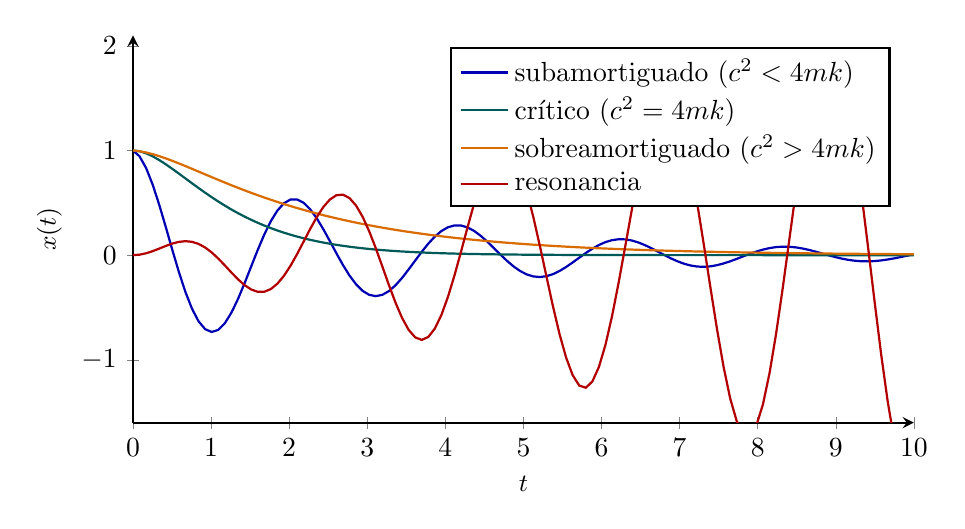
\begin{tikzpicture}
\begin{axis}[
  width=11.5cm, height=6.5cm,
  xlabel={\small $t$}, ylabel={\small $x(t)$},
  domain=0:10, samples=120,
  ymin=-1.6, ymax=2.1, xmin=0, xmax=10,
  legend pos=north east, legend cell align=left,
  axis lines=left, thick, no markers,
]
\addplot[blue!70!black]{exp(-0.3*x)*cos(deg(3*x))}; \addlegendentry{subamortiguado ($c^2<4mk$)}
\addplot[teal!70!black]{(1+1.5*x)*exp(-1.5*x)}; \addlegendentry{crítico ($c^2=4mk$)}
\addplot[orange!85!black]{1.3*exp(-0.5*x)-0.3*exp(-2*x)}; \addlegendentry{sobreamortiguado ($c^2>4mk$)}
\addplot[red!70!black]{0.22*x*sin(deg(3*x))}; \addlegendentry{resonancia}
\end{axis}
\end{tikzpicture}
\caption{Los cuatro comportamientos del oscilador \(mx''+cx'+kx=F(t)\): subamortiguado (oscila y decae), crítico y sobreamortiguado (decaen sin oscilar), y resonancia (amplitud creciente cuando la forzante coincide con la frecuencia natural \(\omega_0=\sqrt{k/m}\)).}
\label{fig:regimenes_amortiguamiento}
\end{figure}

\subsection{Circuitos RLC en serie}

Para un circuito con resistencia $R$, inductancia $L$, capacitancia $C$ y fuerza electromotriz $E(t)$, la carga $Q(t)$ en el capacitor satisface
\[
L Q'' + R Q' + \frac{1}{C} Q = E(t).
\]
Esta ecuación es \emph{formalmente idéntica} a la del oscilador mecánico, con las correspondencias $m\leftrightarrow L$, $c\leftrightarrow R$, $k\leftrightarrow 1/C$ y $F\leftrightarrow E$ (Figura~\ref{fig:circuito_rlc}). Todo lo dicho sobre amortiguamiento y resonancia se traslada palabra por palabra al circuito.

\begin{figure}[H]
\centering
\begin{circuitikz}[american, scale=0.95, transform shape]
\draw (0,0) to[sinusoidal voltage source, l=$E(t)$] (0,2.6)
      to[R, l=$R$] (2,2.6)
      to[L, l=$L$] (4,2.6)
      to[C, l=$C$] (4,0) -- (0,0);
\end{circuitikz}
\caption{Circuito RLC en serie. La carga \(Q(t)\) del capacitor satisface \(LQ''+RQ'+\tfrac{1}{C}Q=E(t)\), análoga a \(mx''+cx'+kx=F(t)\) con \(m\leftrightarrow L\), \(c\leftrightarrow R\), \(k\leftrightarrow 1/C\).}
\label{fig:circuito_rlc}
\end{figure}

\begin{example}[Circuito RLC sin fuente]
Resuelva $Q'' + 4Q' + 20Q = 0$ con $Q(0)=2, Q'(0)=0$.

\begin{myproof}
\textbf{Paso 1.} Característica: $r^2+4r+20=0 \Rightarrow r = -2 \pm 4i$.

\textbf{Paso 2.} $Q(t) = e^{-2t}(c_1 \cos 4t + c_2 \sen 4t)$.

\textbf{Paso 3.} $Q(0)=c_1=2$. $Q'(t)=e^{-2t}[(-2c_1+4c_2)\cos 4t + (-4c_1-2c_2)\sen 4t]$. $Q'(0)=-2c_1+4c_2 = -4+4c_2=0 \Rightarrow c_2=1$.

\textbf{Respuesta final:} $\boxed{Q(t) = e^{-2t}(2\cos 4t + \sen 4t).}$
\end{myproof}
\end{example}

\begin{example}[Circuito RLC con fuente constante (PVI)]
Resuelva $Q''+2Q'+5Q=10$ con condiciones iniciales nulas $Q(0)=0$, $Q'(0)=0$.

\begin{myproof}
\textbf{Paso 1.} Homogénea: $r^2+2r+5=0 \Rightarrow r=-1\pm 2i$, luego $Q_h=e^{-t}(c_1\cos 2t+c_2\sen 2t)$.

\textbf{Paso 2.} Particular constante $Q_p=A$: $5A=10\Rightarrow A=2$ (carga de régimen permanente).

\textbf{Paso 3.} $Q=Q_h+2$. Aplicar $Q(0)=c_1+2=0\Rightarrow c_1=-2$. Derivando, $Q'(0)=-c_1+2c_2=2+2c_2=0\Rightarrow c_2=-1$.

\textbf{Respuesta final:} $\boxed{Q(t)=2-e^{-t}(2\cos 2t+\sen 2t).}$
\end{myproof}
\end{example}

\subsection{Vigas (ecuación de Euler-Bernoulli)}

La deflexión $y(x)$ de una viga sometida a una carga $w(x)$ satisface
\[
EI y'''' = w(x),
\]
donde $E$ es el módulo de Young e $I$ el momento de inercia. Es una EDO de cuarto orden que se resuelve por integración sucesiva.

\begin{example}[Viga en voladizo con carga uniforme]
Resuelva $EI y'''' = w_0$ (constante) con condiciones de extremo empotrado: $y(0)=0, y'(0)=0$ (extremo izquierdo fijo) y extremo libre: $y''(L)=0, y'''(L)=0$.

\begin{myproof}
\textbf{Paso 1.} Integramos cuatro veces:
$y'''' = \frac{w_0}{EI} \Rightarrow y''' = \frac{w_0}{EI}x + C_1$.
$y'' = \frac{w_0}{2EI}x^2 + C_1 x + C_2$.
$y' = \frac{w_0}{6EI}x^3 + \frac{C_1}{2}x^2 + C_2 x + C_3$.
$y = \frac{w_0}{24EI}x^4 + \frac{C_1}{6}x^3 + \frac{C_2}{2}x^2 + C_3 x + C_4$.

\textbf{Paso 2.} Aplicamos $y(0)=0 \Rightarrow C_4=0$; $y'(0)=0 \Rightarrow C_3=0$.
$y''(L)=0 \Rightarrow \frac{w_0}{2EI}L^2 + C_1 L + C_2 = 0$.
$y'''(L)=0 \Rightarrow \frac{w_0}{EI}L + C_1 = 0 \Rightarrow C_1 = -\frac{w_0}{EI}L$.

\textbf{Paso 3.} Sustituimos en $y''(L)$: $\frac{w_0}{2EI}L^2 - \frac{w_0}{EI}L^2 + C_2 = 0 \Rightarrow C_2 = \frac{w_0}{2EI}L^2$.

\textbf{Paso 4.} $y(x) = \frac{w_0}{24EI}x^4 - \frac{w_0 L}{6EI}x^3 + \frac{w_0 L^2}{4EI}x^2$.

\textbf{Respuesta final:} $\boxed{y(x) = \frac{w_0}{24EI}(x^4 - 4L x^3 + 6L^2 x^2).}$
\end{myproof}
\end{example}

\section{Problemas resueltos adicionales}

% Básico
\begin{prob}
Resuelva $y'' - 7y' + 12y = 0$.
\begin{myproof}
$r^2-7r+12=(r-3)(r-4)=0$, $y=c_1 e^{3x}+c_2 e^{4x}$. $\boxed{y=c_1 e^{3x}+c_2 e^{4x}}$
\end{myproof}
\end{prob}

% Básico
\begin{prob}
Resuelva $y'' + 4y' + 4y = 0$.
\begin{myproof}
$(r+2)^2=0$, $y=c_1 e^{-2x}+c_2 x e^{-2x}$. $\boxed{y=e^{-2x}(c_1+c_2 x)}$
\end{myproof}
\end{prob}

% Básico
\begin{prob}
Resuelva $y'' + 2y' + 10y = 0$.
\begin{myproof}
$r=-1\pm 3i$, $y=e^{-x}(c_1 \cos 3x + c_2 \sen 3x)$. $\boxed{y=e^{-x}(c_1\cos 3x+c_2\sen 3x)}$
\end{myproof}
\end{prob}

% Intermedio
\begin{prob}
Resuelva $y''' - 6y'' + 12y' - 8y = 0$.
\begin{myproof}
$(r-2)^3=0$, $y=e^{2x}(c_1+c_2 x+c_3 x^2)$. $\boxed{y=e^{2x}(c_1+c_2 x+c_3 x^2)}$
\end{myproof}
\end{prob}

% Intermedio
\begin{prob}
Resuelva $y'' - y' - 2y = 6x^2$.
\begin{myproof}
Homogénea: $r^2-r-2=(r-2)(r+1)=0$, $y_h=c_1 e^{2x}+c_2 e^{-x}$. Proponemos $y_p=Ax^2+Bx+C$. Derivando y sustituyendo: $-2A x^2 + (-2A-2B)x + (2A - B - 2C) = 6x^2$. Resolviendo: $A=-3, B=3, C=-9/2$. $\boxed{y=c_1 e^{2x}+c_2 e^{-x}-3x^2+3x-\frac{9}{2}}$
\end{myproof}
\end{prob}

% Intermedio
\begin{prob}
Resuelva $y'' + 2y' = 4e^{-2x}$.
\begin{myproof}
Homogénea: $r(r+2)=0$, $y_h=c_1+c_2 e^{-2x}$. $g=e^{-2x}$ solapa; proponemos $y_p=A x e^{-2x}$. Sustituyendo: $-4A e^{-2x}+4A x e^{-2x}+2(A e^{-2x}-2A x e^{-2x})= -2A e^{-2x}=4e^{-2x} \Rightarrow A=-2$. $\boxed{y=c_1+c_2 e^{-2x}-2x e^{-2x}}$
\end{myproof}
\end{prob}

% Intermedio
\begin{prob}
Resuelva $y'' - 4y' + 4y = e^{2x}\cos x$.
\begin{myproof}
Homogénea: $(r-2)^2=0$, $y_h=e^{2x}(c_1+c_2 x)$. $g=e^{2x}\cos x$ no solapa, proponemos $y_p=e^{2x}(A\cos x+B\sen x)$. Con $f=A\cos x+B\sen x$ se tiene $y_p''-4y_p'+4y_p=e^{2x}f''=e^{2x}(-A\cos x-B\sen x)$. Igualando a $e^{2x}\cos x$: $A=-1$, $B=0$. $\boxed{y=e^{2x}(c_1+c_2 x)-e^{2x}\cos x}$
\end{myproof}
\end{prob}

% Desafiante
\begin{prob}
Resuelva $y'' - 3y' + 2y = \frac{e^{2x}}{1+e^x}$ (variación).
\begin{myproof}
$y_1=e^x, y_2=e^{2x}, W=e^{3x}$. $u_1'=-\frac{g y_2}{W}=-\frac{e^{2x}/(1+e^x)\cdot e^{2x}}{e^{3x}}=-\frac{e^{x}}{1+e^x}$; $u_2'=\frac{g y_1}{W}=\frac{e^{2x}/(1+e^x)\cdot e^x}{e^{3x}}=\frac{1}{1+e^x}$. Integrando: $u_1=-\ln(1+e^x)$; $u_2=\ln(e^x)-\ln(1+e^x)=x-\ln(1+e^x)$. $y_p=-e^x\ln(1+e^x)+e^{2x}(x-\ln(1+e^x))$. $\boxed{y=c_1e^x+c_2e^{2x}+e^{2x}x-e^x(1+e^x)\ln(1+e^x)}$
\end{myproof}
\end{prob}

% Intermedio
\begin{prob}
Resuelva $x^2 y'' - 3x y' + 4y = 0$ (raíces repetidas).
\begin{myproof}
$m(m-1)-3m+4=m^2-4m+4=(m-2)^2$, $y=x^2(c_1+c_2\ln x)$. $\boxed{y=x^2(c_1+c_2\ln x)}$
\end{myproof}
\end{prob}

% Intermedio
\begin{prob}
Resuelva $x^2 y'' + x y' + 4y = 0$ (complejas).
\begin{myproof}
$m^2+4=0 \Rightarrow m=\pm 2i$, $y=c_1\cos(2\ln x)+c_2\sen(2\ln x)$. $\boxed{y=c_1\cos(2\ln x)+c_2\sen(2\ln x)}$
\end{myproof}
\end{prob}

% Desafiante
\begin{prob}
Resuelva la EDO no homogénea de Cauchy-Euler: $x^2 y'' - x y' + y = x$.
\begin{myproof}
Homogénea: $m(m-1)-m+1=(m-1)^2$, $y_h=x(c_1+c_2\ln x)$. Por variación de parámetros con $y_1=x$, $y_2=x\ln x$, $W=x$ y la forma estándar $y''-\frac{1}{x}y'+\frac{1}{x^2}y=1/x$ (es decir $g=1/x$): $u_1'=-\frac{(1/x)(x\ln x)}{x}=-\frac{\ln x}{x}$; $u_2'=\frac{(1/x)(x)}{x}=1/x$. Integrando: $u_1=-\frac{1}{2}(\ln x)^2$, $u_2=\ln x$. $y_p= -\frac{x}{2}(\ln x)^2 + x(\ln x)^2 = \frac{x}{2}(\ln x)^2$. $\boxed{y=x(c_1+c_2\ln x)+\frac{x}{2}(\ln x)^2}$
\end{myproof}
\end{prob}

% Intermedio
\begin{prob}
Oscilador amortiguado: $x''+6x'+25x=0$, condiciones $x(0)=0, x'(0)=1$.
\begin{myproof}
$r^2+6r+25=0 \Rightarrow r=-3\pm 4i$, $x=e^{-3t}(c_1\cos 4t+c_2\sen 4t)$. $x(0)=c_1=0$. $x'(0)= -3c_1+4c_2=4c_2=1 \Rightarrow c_2=1/4$. $\boxed{x=\frac{1}{4}e^{-3t}\sen 4t}$
\end{myproof}
\end{prob}

% Desafiante
\begin{prob}
Resuelva $y'' + 2y' + y = e^{-x}\ln x$ (variación).
\begin{myproof}
$y_1=e^{-x}, y_2=x e^{-x}, W=e^{-2x}$. $g=e^{-x}\ln x$. $u_1'=-\frac{e^{-x}\ln x \cdot x e^{-x}}{e^{-2x}}=-x\ln x$; $u_2'=\frac{e^{-x}\ln x \cdot e^{-x}}{e^{-2x}}=\ln x$. Integrando: $u_1=-\frac{x^2}{2}\ln x+\frac{x^2}{4}$; $u_2=x\ln x-x$. $y_p=(-\frac{x^2}{2}\ln x+\frac{x^2}{4})e^{-x} + (x\ln x-x)x e^{-x} = e^{-x}(\frac{x^2}{4}+\frac{x^2}{2}\ln x - x^2) = e^{-x}(\frac{x^2}{2}\ln x - \frac{3x^2}{4})$. $\boxed{y=e^{-x}(c_1+c_2x)+\frac{x^2}{4}e^{-x}(2\ln x-3)}$
\end{myproof}
\end{prob}

% Desafiante
\begin{prob}
Resuelva $y'' - y = \frac{2e^x}{e^x+1}$ (variación).
\begin{myproof}
$y_1=e^x, y_2=e^{-x}, W=-2$. $g=2e^x/(e^x+1)$. $u_1'=-\frac{g y_2}{W}=\frac{1}{e^x+1}$; $u_2'=\frac{g y_1}{W}=-\frac{e^{2x}}{e^x+1}$. Integrando (nota: $\frac{d}{dx}[x-\ln(e^x+1)]=\frac{1}{e^x+1}$): $u_1=x-\ln(e^x+1)$; $u_2=-\int\frac{e^{2x}}{e^x+1}dx=-\int\!\left(e^x-1+\frac{1}{e^x+1}\right)dx=-(e^x-\ln(e^x+1))=-e^x+\ln(e^x+1)$. $y_p=(x-\ln(e^x+1))e^x+(-e^x+\ln(e^x+1))e^{-x}=xe^x-(e^x-e^{-x})\ln(e^x+1)-1$. $\boxed{y=c_1e^x+c_2e^{-x}+xe^x-(e^x-e^{-x})\ln(e^x+1)-1}$
\end{myproof}
\end{prob}

\section{Problemas propuestos}

% Básico
\begin{prob}
Resuelva $y'' - y' - 6y = 0$.
\end{prob}

\begin{prob}
Resuelva $y'' + 6y' + 9y = 0$.
\end{prob}

\begin{prob}
Resuelva $y'' + 4y = 0$.
\end{prob}

\begin{prob}
Resuelva $y'' - 2y' + 5y = 0$.
\end{prob}

% Intermedio
\begin{prob}
Resuelva $y''' - y' = 0$.
\end{prob}

\begin{prob}
Resuelva $y'' - 3y' + 2y = 4x$ (coeficientes indeterminados).
\end{prob}

\begin{prob}
Resuelva $y'' + y = 4e^x$.
\end{prob}

\begin{prob}
Resuelva $y'' - 4y = e^{2x}$ (atención al solapamiento con la homogénea).
\end{prob}

\begin{prob}
Resuelva el PVI $y'' + 2y' + 2y = 0$ con $y(0)=1$, $y'(0)=0$.
\end{prob}

\begin{prob}
Resuelva la ecuación de Cauchy-Euler $x^2 y'' - 2y = 0$.
\end{prob}

\begin{prob}
Resuelva la ecuación de Cauchy-Euler $x^2 y'' + 5x y' + 4y = 0$ (raíces repetidas).
\end{prob}

\begin{prob}
Oscilador forzado sin resonancia: resuelva $x'' + 4x = \cos t$.
\end{prob}

% Desafiante
\begin{prob}
Resuelva $y'' + y = \sec x$ (variación de parámetros).
\end{prob}

\begin{prob}
Resuelva la Cauchy-Euler no homogénea $x^2 y'' - 3x y' + 3y = 2x^4$.
\end{prob}

\begin{prob}
Resonancia: resuelva $x'' + 9x = 2\sen 3t$ e identifique el término cuya amplitud crece con $t$.
\end{prob}